\section{项目的主要内容和技术路线}

\subsection{主要研究内容}

该研究希望统一并比较现有的基于能量函数的安全控制算法,具体来说,即统一并比较现有的四种代表性方法:势能场算法(PFM)\cite{khatib1986real},滑动模式算法(SMA)\cite{gracia2013reactive},屏障函数算法(BFM)\cite{ames2014control},以及安全集算法(SSA)\cite{liu2014control}。

该项目主要包括三个部分:

1、提出数学框架并证明现有方法可以融入到该框架之中。

2、编写基准评测平台,实现多种复杂环境下的人机交互测试并测试现有算法。

3、根据理论分析与实验结果,改进现有算法。

\subsubsection{数学框架}

该研究希望能够提出一个提出数学框架并证明以上方法可以融入到该框架之中,能够被视作是统一框架应用了不同超参数后的不同形式。

\subsection{技术路线}

该项目中需要的数学工具主要有:高等代数、线性代数、机器人运动学及逆运动学、凸优化。

编程部分由Python语言实现,需要的技术有:图形化界面编写,机器人运动学模型实现,现有算法实现。

\subsection{可行性分析}

\subsubsection{现有算法分析}

\begin{figure}[h]
    \begin{center}
        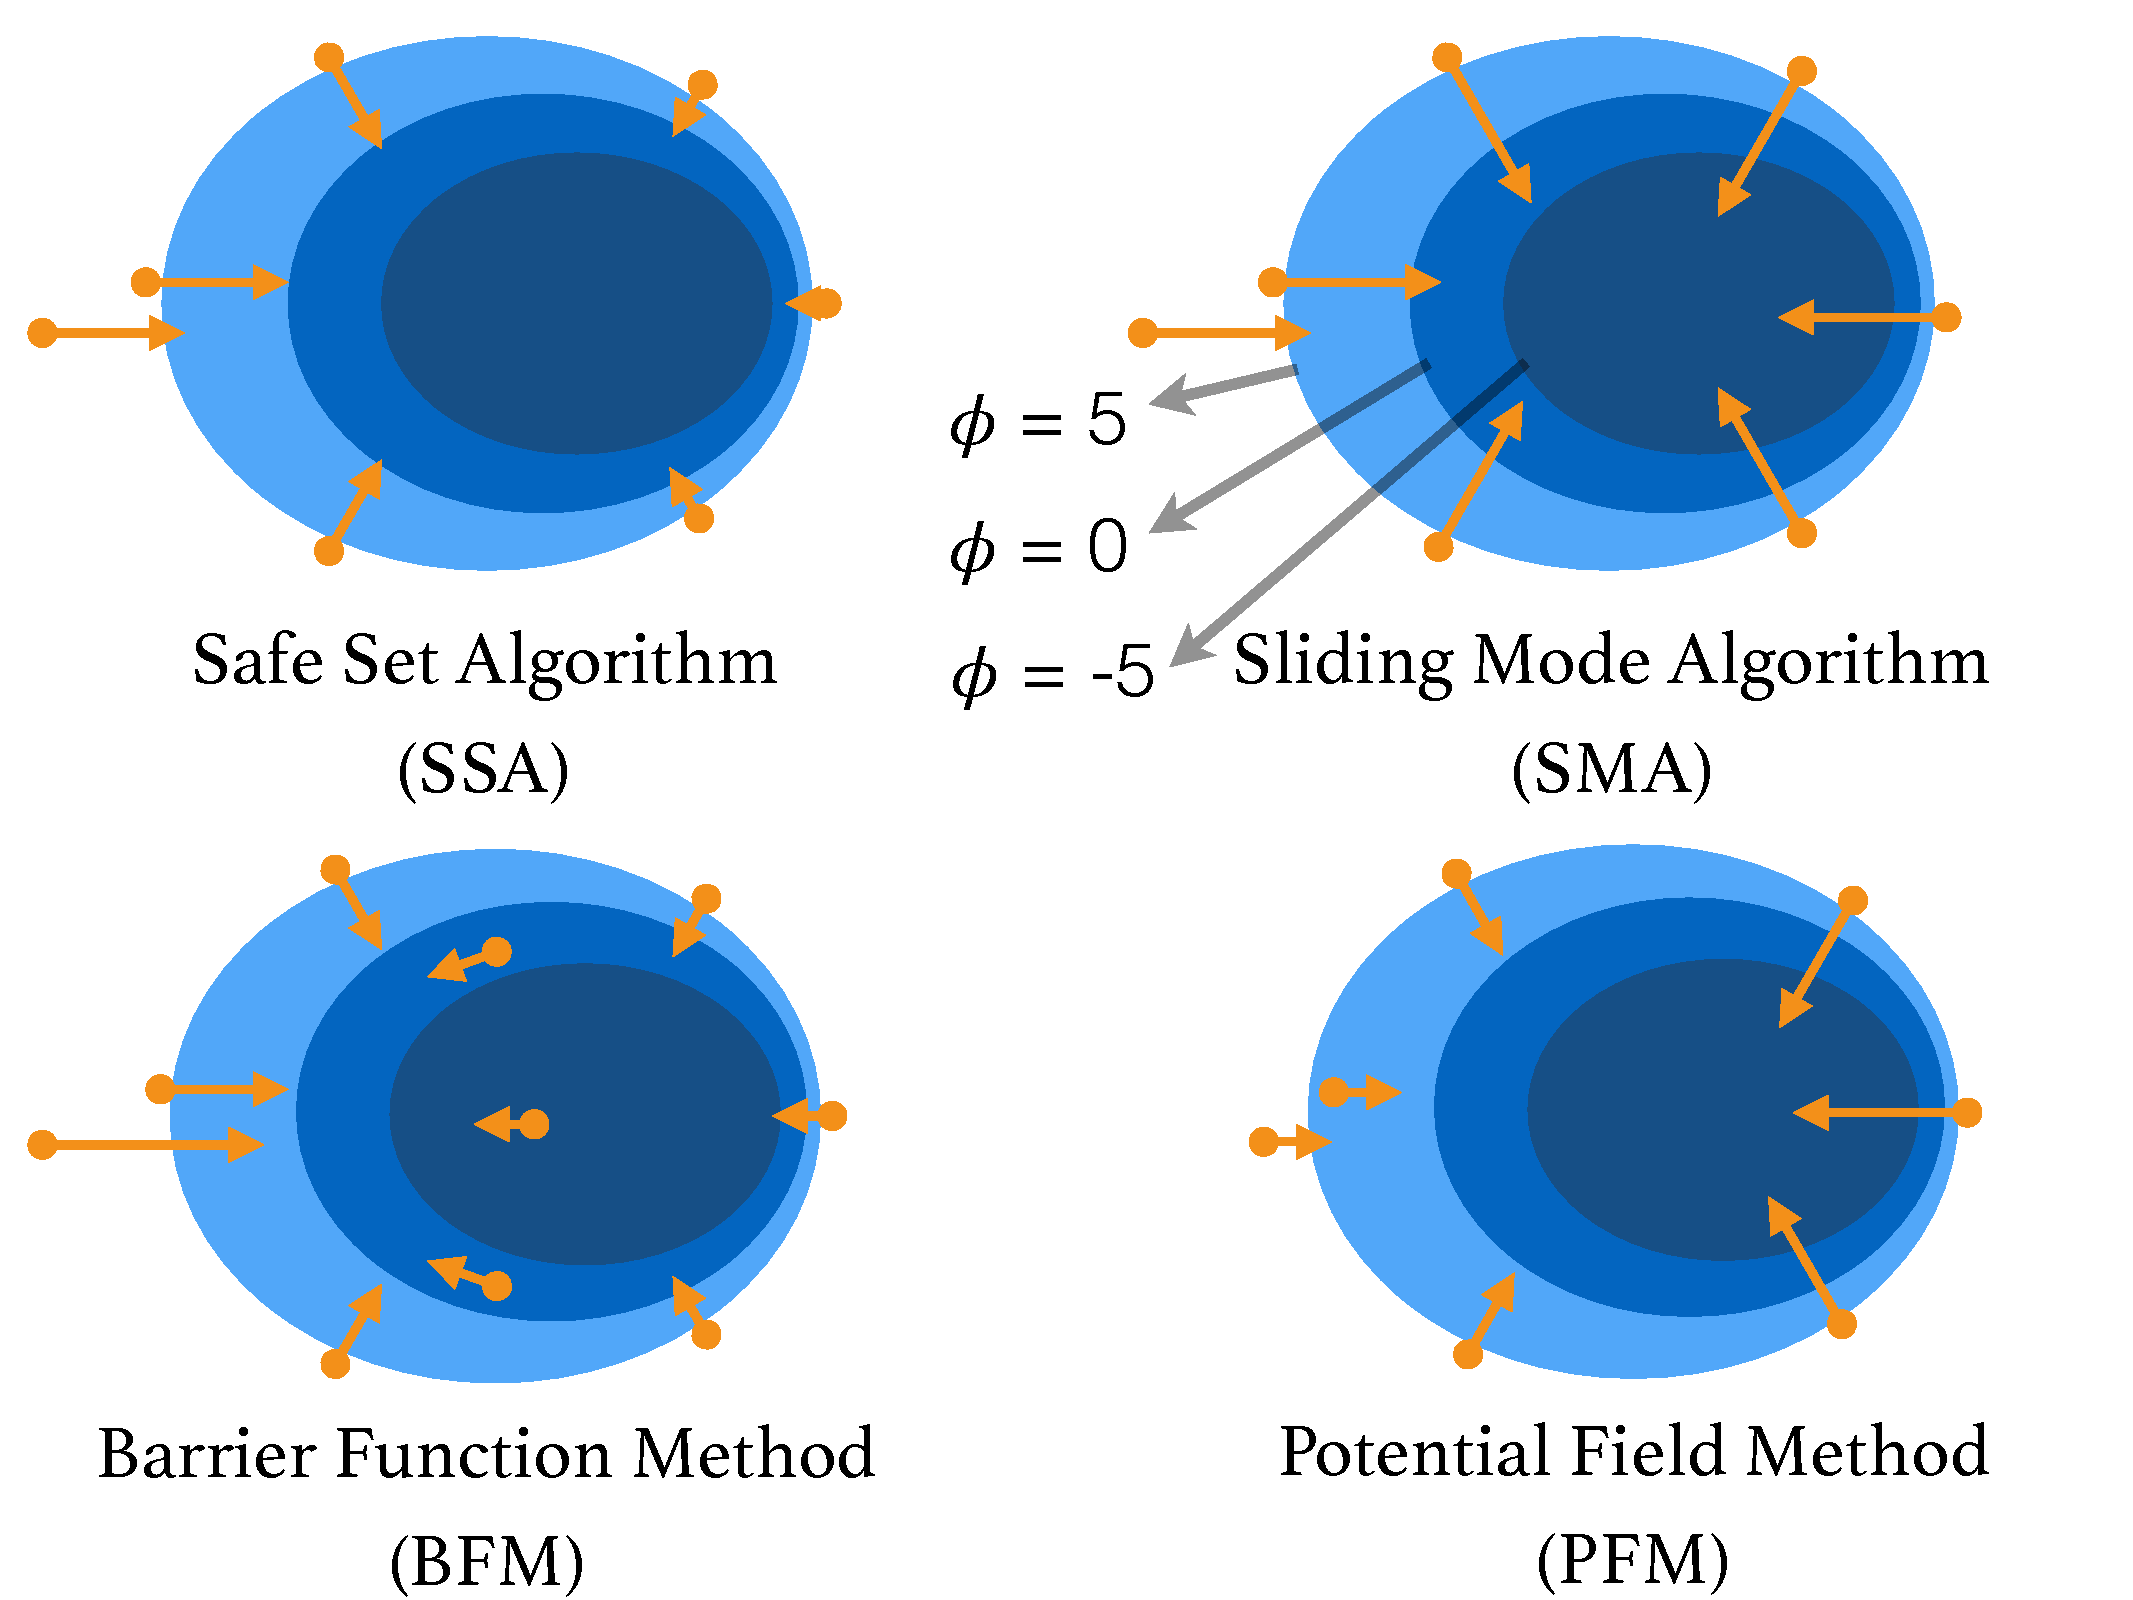
\includegraphics[width=0.8\textwidth]{figure/phase.pdf}%\footnote{For simplicity, the dynamics are assumed to be $\dtv{x} = \v{u}$, while the reference input is assumed to be zero.}
        \caption{四种安全算法的相位图。平面代表状态空间,等高线代表能量函数$\phi$不同的等值线。如果$\phi \leq 0$则该系统处于安全的状态,反之则为危险。圆点代表算法给出控制的状态点,箭头指示的方向为算法给出的控制输入的方向,箭头的长度代表该控制的大小。}
        \label{fig:safe_control}
    \end{center}
\end{figure}

分析现有算法之前我们简要介绍数学标记:

$\phi$代表能量函数,$\nabla \phi$为能量函数的梯度,$\v{u}$表示算法给出的控制输入,$\v{u}_c$为控制输入在笛卡尔坐标系中的表示。$\v{u}_0$是参考输入,如果当前系统处于安全的状态,则可直接采用参考输入作为算法输出。

基于能量函数的安全控制算法具有不同的能量函数定义,而该定义并非与方法相绑定,因此我们可以给他们设定统一的能量函数,以方便我们关注他们的应对策略的不同。

PFM:PFM给出的控制输入与能量函数梯度$\nabla \phi$程正比例关系。PFM并不会在参数空间中直接给出控制输入$\v{u}$,而是在笛卡尔坐标系中给出控制$\v{u}_c$,再由逆运动学转化为参数空间的控制。PFM的控制策略是:
\begin{align}
    % & \phi = \frac{\eta}{2} (\frac{1}{d} - \frac{1}{d_{min}})^2 \\
    & \v{u}_c = \left\{\begin{array}{ll}\v{u}_c^0 - c_1\ \nabla \tilde\phi &\text{if } \tilde\phi \geq 0 \\
    \v{u}_c^0 & \mathrm{otherwise}
    \end{array}\right. \label{eq: pfc},
\end{align}


SMA:SMA给出的控制输入沿着梯度方向,具有固定大小的模长。SMA给出的控制输入是根据能量函数关于控制输入的李导数所得,仅在系统处于危险状态时给出控制输入。其控制策略为:
\begin{align}
    % & \phi = d_{min}^2 - d^2 - k_v\dot d \\
    & \v{u} = \left\{\begin{array}{ll}\v{u}_0 - c_2\ \LgP \transpose &   \text{if } \phi \geq 0 \\
    \v{u}_0 & \mathrm{otherwise}
    \end{array}\right. \label{eq: smc},
\end{align}
$c_2>0$是一个足够大的常数,使得$\dot{\phi} = \LfP - c_2\ \|\LgP\|^2 + \LgP\ \v{u}_0$恒为负数。
%SMA provides a large enough modification of $\v{u}_0$ when $\phi > 0$ to make the state $\v{x}$ go back to safe region.  %to trigger the regulation of maximum control.


SSA:SSA给出的控制输入与能量函数的梯度$\nabla \phi$程反比例关系。当$\phi>0$时,SSA计算得到与参考输入$\v{u}_0$最接近且能够使得能量函数$\phi$降低的控制输入作为输出。其数学描述如下:
\begin{align}\label{eq: SSA}
    % & \phi = d_{min}^2 - d^2 - k_v\dot d \\
    & \v{u} = \min_\v{u} ||\v{u}_0 - \v{u}||_2,\ \st \ \dot \phi\leq \eta \ \text{or}\ \phi < 0,
\end{align}

BFM:BFM在系统处于安全状态时,即$\phi < 0$,仍会给出控制输入。控制输入的模长与能量函数$\phi$及能量函数的梯度$\nabla \phi$均有关。BFM计算得到与参考输入$\v{u}_0$最接近且能够使得能量函数满足$\dtv{\phi} < \lambda\ \v{\phi}$的控制作为输出。$\lambda$为一小于零的常数。其数学描述如下:
\begin{align}\label{eq: BFM}
    % & \phi = \frac{1}{(d - d_{min} + \dot d  t_{react})}\\
    & \v{u} = \min_\v{u} \norm{\v{u}_0 - \v{u}}_2,\ \st\ \dtv{\phi} \leq \lambda\ \v{\phi},
\end{align}

\subsubsection{数学框架可行性}

不难看出,上述方法具有众多相似点,并遵循相似的数学逻辑。因此提炼出他们的共同逻辑作为整体数学框架具有一定可行性。而将他们视作同一框架应用不同超参数后的具体形式,要求我们把不同算法都表示为参数形式。对于不同的决策环境,我们可以使用多种方式来实现连续或离散的决策路线,比如使用sigmoid函数或指示函数等方式,因此数学框架具有较高的可行性。

\subsubsection{基准程序可行性}

基准程序的主要目的是模拟现实中的交互情况,快速大量的测试算法。主要难点在于实现现实中的机器人模型及人类行为模型。机器人模型可以根据动力模型进行仿真,可以得到接近真实的效果。已有许多软件实现了其他场景下类似的功能,该部分可行性较高。人类模型可以考虑使用模仿学习学习人类行为,习得人类行为算法,使用该算法进行仿真。该方法可行性较高。

\subsubsection{改进现有算法}

该部分视理论分析结果与实验结果而定。有较大可能性挖掘出改进空间。